
\chapter{Návrh systému} 
\label{kap:návrh systému}
\pagestyle{fancy}
\fancyhf{}
\fancyfoot[CE,CO]{\thepage}
\renewcommand{\footrulewidth}{1pt}
\lhead{Návrh systému}


\section{Výber kamier}

\subsection{Intel Realsense SR300}

Táto kamera pracuje na princípe SLS a predstavuje vylepšenú verziu staršej Intel RealSense F200. Ide o cenovo dostupnú hĺbkovú kameru, ktorá sníma hĺbku v rozsahu od $0.2-1.5 m$. Poskytuje dynamické snímanie scény pri nízkej spotrebe (napájanie cez USB). V kombinácií s farebným obrazom ($1920\times1080p$, $30Hz$) a hĺbkovou mapou ($640x480p$) ide o jednu z najlepších dostupných SLS kamier na trhu. 

\begin{figure}[H]
	\centering
	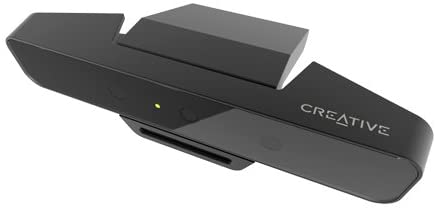
\includegraphics[width=0.7\textwidth]{figures/sr300.jpg}
	\caption{SLS kamera Intel RealSense SR300.}
	\label{fig::sr300}
\end{figure}

Táto kamera obsahuje RGB senzor, IR laserový projektor, IR prijímač a mikrofón. Detailnejšie opísanie princípu SLS je v podkapitole \ref{sec:sls}.

\subsection{Microsoft Kinect v2}

Ide o druhú generáciu hĺbkových kamier od spoločnosti Microsoft. Oproti prvej generácií využíva technológiu ToF (detailnejšie v \ref{sec:tof}), pričom ide o jednu z najznámejších senzorov tohto typu na svete. Rozsah snímanej scény je $0.5-4.5 m$. Farebný obraz je dodávaný v rozlíšení $1920\times1080p$ a $30Hz$, hĺbková mapa ma rozlíšenie $512\times424$.

\begin{figure}[H]
	\centering
	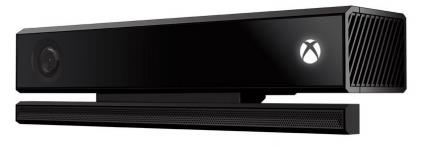
\includegraphics[width=0.7\textwidth]{figures/kinect.png}
	\caption{ToF kamera Microsoft Kinect v2.}
	\label{fig::kinect}
\end{figure}

Presnosť hĺbkovej mapy je oproti prvej verzii Kinectu vyššia, taktiež je znížený negatívny vplyv spôsobovaný slnečným svetlom.


\subsection{Porovnanie presnosti kamier}

Cieľom testovania bolo porovnať presnosť 3D rekonštrukcie statického objektu pre kamery Intel RealSense SR300 a Microsoft Kinect v2. Pomocou programov, určených k práci s jednotlivými kamerami, bola vytvorená séria snímok hĺbkových máp a ich rekonštruovaných 3D modelov. Pred snímaním bola vykonaná geometrická kalibrácia kamier, ktorej technické detaily sú opísané v kapitole \ref{sec:kinect_calib}. Kalibrovanými kamerami sa následne z 3 uhlov (pohľady spredu, z ľavej a pravej strany) získali ich 3D rekonštrukcie, ktoré zachytávali všetky potrebné detaily pre meranie. Identické natočenie pre obe kamery bolo zabezpečené rotačným podstavcom. 

\begin{figure}[H]
	\centering
	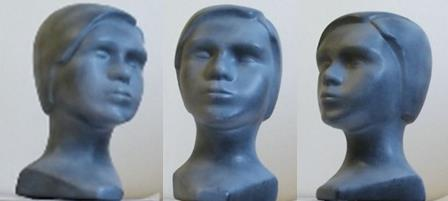
\includegraphics[width=0.7\textwidth]{figures/rgb_compar.png}
	\caption{ToF kamera Microsoft Kinect v2.}
	\label{fig::rgb_compare}
\end{figure}

Povrch objektu bol špeciálne upravený, aby nevytváral odlesky spôsobujúce zhoršovanie rekonštruovaného 3D modelu. 

\section{Snímanie dynamických objektov}

Pri snímaní dynamických objektov je potrebné uvažovať so vznikom pohybových artefaktov. Tie vznikajú, ak objekt v dobe skenovania mení svoje priestorové umiestnenie. Z toho dôvodu je potrebné buď stabilizovať objekt počas doby snímania alebo redukovať časovú dĺžku skenovania. Keďže tento systém má byť určený pre medicínske aplikácie, kde skenovaný objekt bude pediatrický pacient, je potrebné overiť možnosti experimentálne.


\subsection{Jedno-kamerové snímanie dynamických objektov}

Experimentálne snímanie pacientov bolo vykonávané na Klinike detí a dorastu Jesseniovej lekárskej fakulty v Martine, Laboratórium spánkovej medicíny. Do testu bolo vybraných 9 pacientov rôzneho pohlavia,vo vekovom rozmedzí od 4 do 12 rokov. 

Ako skenovací nástroj bola použitá kamera Kinect v2. V spolupráci s komerčným softvérom KScan3D boli vytvorené modely pacientov, ktoré sú zobrazené na obr. \ref{fig:dynamic_patient:a} a \ref{fig:dynamic_patient:b}. 

\begin{figure}[H]
	\centering
	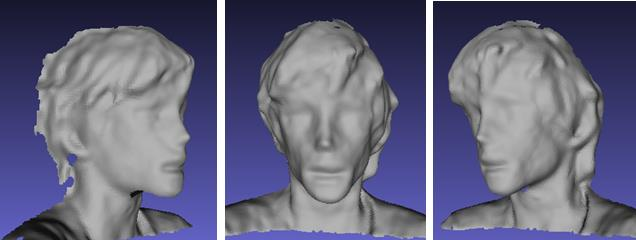
\includegraphics[width=\textwidth]{figures/dynamic_patient_a.png}
	\caption{ToF kamera Microsoft Kinect v2.}
	\label{fig:dynamic_patient:a}
\end{figure}

\begin{figure}[H]
	\centering
	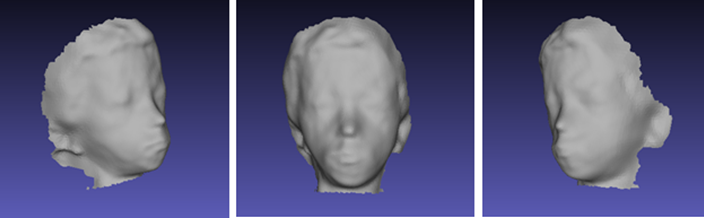
\includegraphics[width=\textwidth]{figures/dynamic_patient_b.png}
	\caption{Úkažka .}
	\label{fig:dynamic_patient:b}
\end{figure}

Ako je vidieť, modely sú nekvalitné a výrazne deformované. Je to spôsobené tým, že objekty nedokázali zostať v statickej polohe počas doby skenovania (tá presahovala 1 minútu pri každom pacientovi). Tendenciou bolo otáčať sa za kamerou, čo viac krát viedlo k nutnosti začas celý proces od znova. 

Takéto modely nie su postačujúce pre diagnostikovanie OSAS. Ich miera nepresnosti je veľmi vysoká a užitočná geometria tváre sa stráca. Z experimentu vyplýva, že jedno-kamerový systém je nepoužiteľný pre skenovanie dynamických objektov ako sú pediatrickí pacienti.  

\subsection{Priestorové rozloženie multi-kamerového systému}

Pri multi-kamerovom systéme sa pre skenovanie používajú viaceré kamery, ktoré su staticky rozložene v priestore. Ich počet závisí od detailov objektu, ktoré majú byť zosnímané.

\begin{figure}[H]
	\centering
	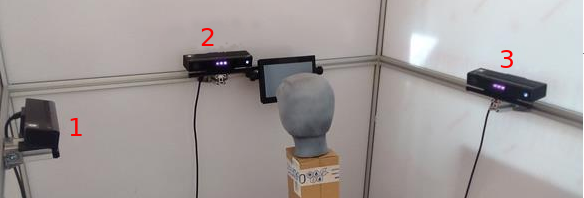
\includegraphics[width=0.6\textwidth]{figures/multicam_placement.png}
	\caption{Úkažka .}
	\label{fig:multicam:placement}
\end{figure}


Medzi hlavné požiadavky na model sú: hlava musí obsahovať laterálne pohľady (umožniť prekrytie s cefalometrickou snímkou) a orientačné bodov mäkkého tkaniva. Dôležité je aj získanie informácie o šírke krk. Na obrázku \ref{fig:multicam:placement} je zobrazené rozloženie kamier v skenovacej kabíne. Ich jednotlivé 3D modely aj s verifikáciou požiadaviek sa nachádzajú na obr. \ref{fig:multicam:models}. 

\begin{figure}[H]
	\centering
	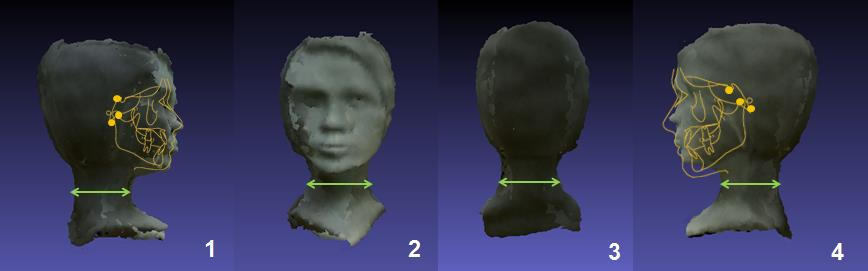
\includegraphics[width=\textwidth]{figures/multicam_placement_scans.png}
	\caption{Úkažka .}
	\label{fig:multicam:models}
\end{figure}

\subsection{Sekvenčné snímanie multi-kamerového systému}

Sekvenčný mód predstavuje postupné snímanie. V jednom momente vždy sníma len jedna kamera ostatné kamery sú vypnuté. Tento režim je pri ToF kamerách často využívaný, pretože tu nevzniká multi-kamerová interferencia. Problémom je však dlhá doba zapínania IR projektora, ktorá pri kamerách Microsoft Kinect v2 dosahuje približne $1s$. Časový odstup medzi dvoma prijatými snímkami je pri $30Hz$ okolo $33ms$.

\subsection{Paralelné snímanie multi-kamerového systému}

V paralelnom režime pracujú všetky kamery v rovnakom čase. Oproti sekvenčnému snímaniu sa inicializácia vykonáva pre každú kameru iba raz. Tým sa radikálne znižuje doba snímania objektu zo všetkých uhlov. Nevýhodou je ale vznik multi-kamerovej interferencie, ktorá dokáže negatívne ovplyvniť výstupné hĺbkové mapy. Časový rozostup medzi jednotlivými snímkami je ovplyvnení samotným spracovaním dát, maximálne však $33ms$ medzi všetkými snímkami. 

\subsection{Porovnanie režimov snímania dynamických objektov}

Pre porovnanie týchto režimov bol navrhnutý experiment, pri ktorom sa porovná veľkosť zmeny polohy objektu v závislosti na dĺžke snímania. Pre testovanie bol vyrobený merací prvok, ktorý pozostával z jednosmerného motora, ukazovateľa aktuálnej polohy a statického podstavca slúžiaceho ako uhlomer. Na hriadeli motora bol pripevnený ukazovateľ, ktorý vykonával pohyb po kružnici. Rýchlosť bola nastavená na regulovateľným zdrojom tak, aby otočka trvala $5s$. Obvod statického podstavca bol rozdelený na 36 dielov oddelených od seba po $10^\circ$. Kvôli identifikácii polohy podstavec obsahoval zvýraznený nultý bod a šípku informujúcu o smere otáčania ukazovateľa.  

\begin{figure}[h]
	\centering
	\begin{subfigure}[b]{\textwidth}
		\centering
		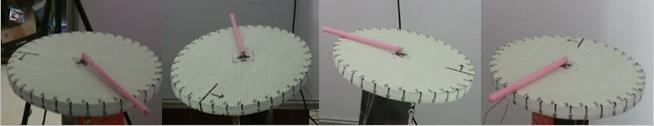
\includegraphics[width=\textwidth]{figures/dynamic_sequence.png}
		\label{fig:dynamic:sequence}
	\end{subfigure}
	\vfill
	\begin{subfigure}[b]{\textwidth}
		\centering
		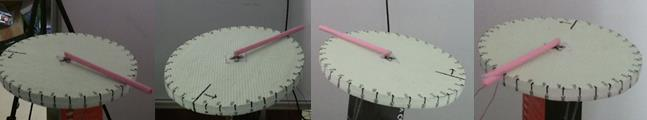
\includegraphics[width=\textwidth]{figures/dynamic_parallel.png}
		\label{fig:dynamic:parallel}
	\end{subfigure}
	\caption{}
	\label{fig:dynamic:results}
\end{figure}

Pri sekvenčnom režime boli snímky z kamier získavané postupne od 1 po 4 kameru. Pri paralelnom režime je ťažké identifikovať poradie. Pre porovnanie bolo potrebné získané hĺbkové mapy previesť na mračno bodov a pomocou ICP metódy ich registrovať do jedného modelu (zhodná pozícia nultého bodu). 

\begin{figure}[h]
	\centering
	\begin{subfigure}[b]{0.42\textwidth}
		\centering
		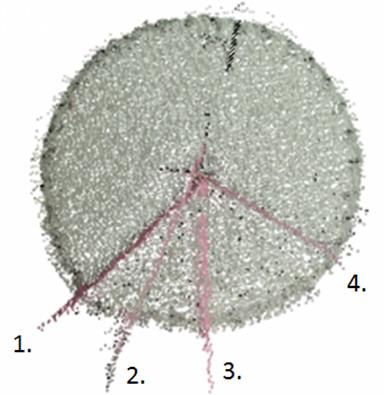
\includegraphics[width=\textwidth]{figures/dynamic_result_seq.png}
		\caption{}
		\label{fig:depthir:a}
	\end{subfigure}
	\hfill
	\begin{subfigure}[b]{0.42\textwidth}
		\centering
		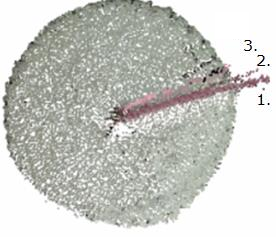
\includegraphics[width=\textwidth]{figures/dynamic_result_par.png}
		\caption{}
		\label{fig:depthir:b}
	\end{subfigure}
	\caption{Obrazy z senzora Microsoft Kinect v2: (\textbf{a}) IR obraz bez interferencie. (\textbf{b}) IR obraz s interferenciou. (\textbf{c}) Hĺbková mapa IR obrazu (a). (\textbf{d}) Hĺbková mapa IR obrazu (b). Miesto interferencie je zvýraznené červenou farbou.}
	\label{fig:depthir}
\end{figure}

Z výsledných modelov je jasne vidieť, že paralelné spracovanie dát má vyšší zmysel pri snímaní dynamických objektov. Pri sekvenčnom režime je rozdiel polohy ukazovateľa výrazný, čo spôsobovalo problémy aj pri ICP registrácií. Naproti tomu je model vytvorený paralelným režimom konzistentnejší, rozdiel polohy ukazovateľa je podstatne menší. Ten by sa dal znížiť hardvérovým synchronizovaným snímaním. Pri kamerách Kinect v2 však táto možnosť chýba.

\section{Kalibrácia kamier systému}
\label{sec:kinect_calib}
Pre kalibráciu bol použitý \textit{Matlab Calibration ToolBox}. 

\subsection{Geometricka kalibrácia}
Cieľom geometrickej kalibrácie je získanie vnútorných parametrov  kamery spolu s korekčnými parametrami pre odstránenie tangenciálneho a radiálneho skreslenia. Tieto parametre bolo potrebne získať pre RGB aj IR senzory všetkých používaných hĺbkových kamier Kinect v2. 

Pre kalibráciu RGB a IR senzora sa vytvorila séria snímok, ktoré  obsahovali kalibračný vzor snímaný z rôznych uhlov. Ten bol reprezentovaný šachovnicovým motívom o rozmeroch $10\times8$, pričom dĺžka hrany mala veľkosť $36mm$.


%\begin{figure}[h]
%	\centering
%	\begin{subfigure}[b]{0.59\textwidth}
%		\centering
%		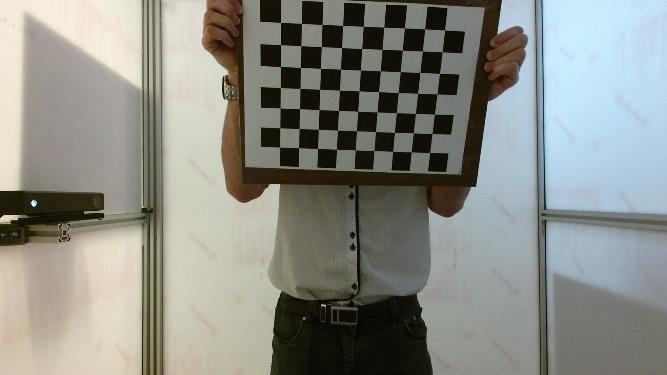
\includegraphics[width=\textwidth]{figures/calibration_rgb.png}
%		\caption{}
%		\label{fig:calib:rgb}
%	\end{subfigure}
%	\hfill
%	\begin{subfigure}[b]{0.4\textwidth}
%		\centering
%		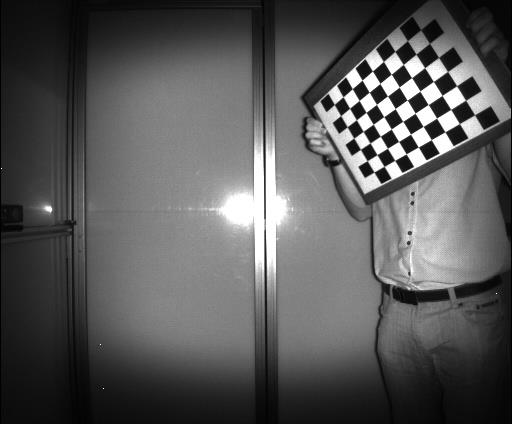
\includegraphics[width=\textwidth]{figures/calibration_ir.png}
%		\caption{}
%		\label{fig:calib:ir}
%	\end{subfigure}
%	\caption{Obrazy z senzora Microsoft Kinect v2: (\textbf{a}) IR obraz bez interferencie. (\textbf{b}) IR obraz s interferenciou. (\textbf{c}) Hĺbková mapa IR obrazu (a). (\textbf{d}) Hĺbková mapa IR obrazu (b). Miesto interferencie je zvýraznené červenou farbou.}
%	\label{fig:calib:single}
%\end{figure}

Pre overenie správnosti kalibrácie IR snímača sa porovnával kalibrovaný kamerový systém s nekalibrovaným voči referenčnému modelu. Pri rovnakých podmienkach prostredia bol zosnímaný model hlavy s továrenskými nastaveniami, potom boli použité kalibračné koeficienty získané v predchádzajúcom kroku. Referenčný model bol vytvorený ručným laserovým skenerom. Ukážky sa nachádzajú na obr. \ref{fig:calib:models}. 

\begin{figure}[H]
	\centering
	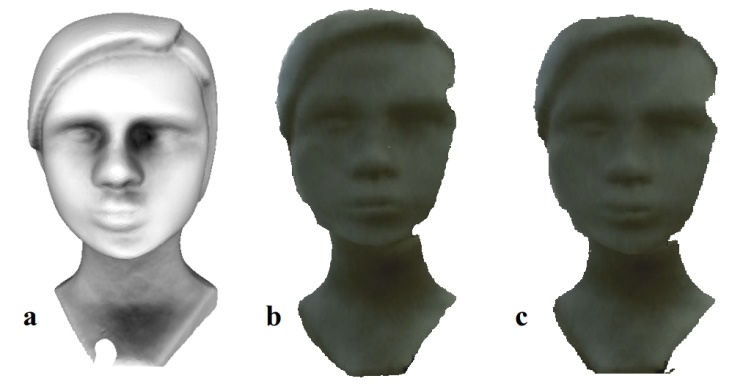
\includegraphics[width=0.6\textwidth]{figures/calibration_models.jpg}
	\caption{}
	\label{fig:calib:models}
\end{figure}

Porovnanie priestorovej rekonštrukcie hĺbkových máp bolo robené pomocou Hausdorffovej vzdialenosti. V nej je detailnejšie zobrazené, aký vplyv má kalibrácia na generované dáta. Z modelu vzdialenosti (obr. \ref{fig:calib:haus:single}) je vidieť, že nekalibrovaný systém vykazoval vyššiu chybu na okrajoch modelu. To je spôsobené pozitívnym radiálnym skreslením IR senzora, ktorého intenzita je výraznejšia na okrajoch obrazu. Štatistické výsledky pre 10 modelov sa nachádzajú v tabuľke \ref{tab:calib:single}.

\begin{figure}[H]
	\centering
	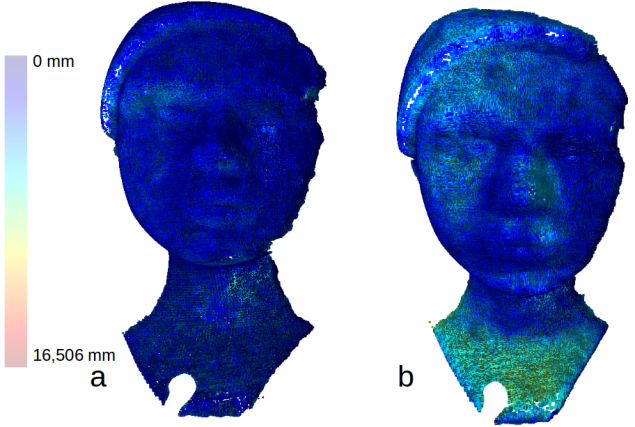
\includegraphics[width=0.52\textwidth]{figures/calibration_hausdorff_single.jpg}
	\caption{}
	\label{fig:calib:haus:single}
\end{figure}



\begin{table}[h]
	\caption{\label{tab:calib:single} Štatistické porovnanie geometrickej kalibrácie kamier }
	\centering
	\begin{tabular}{cccc}
		\toprule
		\textbf{Model} & \textbf{Počet bodov [-]} & \textbf{Mean [mm]} & \textbf{RMS [mm]} \\ 
		\midrule
		\textbf{Nekalibrovaný} & 185187 & 3,0206	& 3,8444 \\
		\textbf{Kalibrovaný} & 296585   & 2,1832   & 2,9506  \\  
		\bottomrule
	\end{tabular}
\end{table}

Týmto krokom sa overil spôsob geometrickej kalibrácie hĺbkových máp. V systéme, kde sa využíva viacero kamier a je kladený dôraz na precíznosť rekonštrukcie, ide o nevyhnutný krok. 


\subsection{Multi-kamerová kalibrácia}

V tomto procese sa hľadajú vzájomné pozície kamier vo svetovej súradnicovej sústave. Ich vzájomnú pozíciu určujú rotačné a translačné parametre (kombinácia afinných transformácií z kapitoly \ref{sec:afine}). Tie je možné získať viacerými spôsobmi. Dôležité je si určiť referenčnú kameru, ktorej matica vonkajších parametrov bude mať tvar identickej afinnej transformácie. Pri multi-kamerovej kalibrácií sa využíva podobný postup ako pri geometrickej kalibrácii. Rozdielom je však, že sa kalibračný vzor sníma súčasne z viacerých kamier. Problém nastáva, ak ich rozloženie neumožňuje súčasné snímanie. Takýto prípad je zachytený na obr. \ref{fig:multicam:placement}.

Riešením je separátne kalibrovanie medzi susednými kamerami (napr. 1-2, 1-3 a 2-4 alebo 3-4). 

\begin{figure}[H]
	\centering
	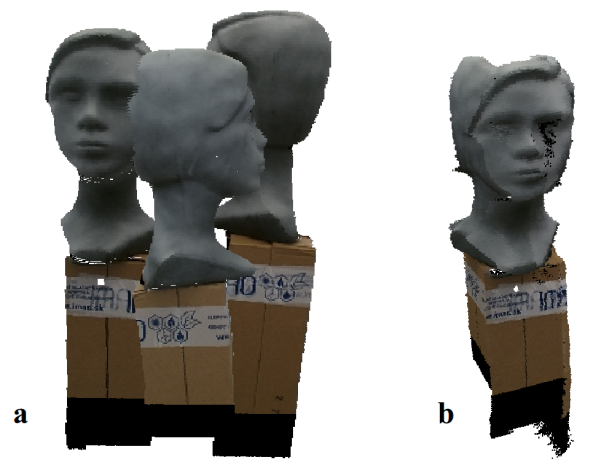
\includegraphics[width=0.52\textwidth]{figures/calibration_multi.jpg}
	\caption{}
	\label{fig:calib:haus:single}
\end{figure}

\begin{figure}[H]
	\centering
	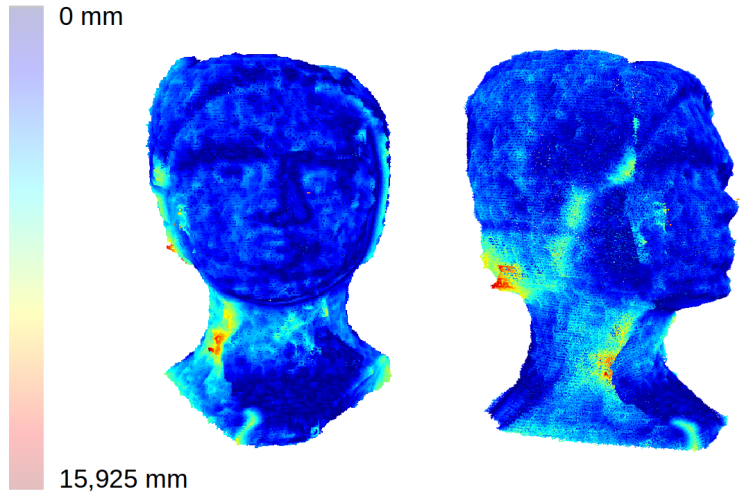
\includegraphics[width=0.52\textwidth]{figures/calibration_hausdorff_multi.jpg}
	\caption{}
	\label{fig:calib:haus:single}
\end{figure}


\begin{equation}
\label{eq:multi:calib:a}
\begin{aligned}
\begin{bmatrix}
1 & 0 & 0 & 0 \\
0 & 1 & 0 & 0 \\
0 & 0 & 1 & 0 \\
0 & 0 & 0 & 1 
\end{bmatrix}, 
\begin{bmatrix}
1 & -0.03 & 0.06 & -0.03 \\
0.02 & 1 & 0.07 & -0.04 \\
-0.06 & -0.06 & 1 & 0.02 \\
0 & 0 & 0 & 1 
\end{bmatrix}
\end{aligned}
\end{equation}




\section{Návrh algoritmu}


\subsection{Paralelné spracovanie dát}

\subsection{Analýza pohybu objektu}

\subsection{ICP registrácia}

\subsection{Segmentácia hĺbkovej mapy}
